\subsection{Pros and Cons}\label{sec:ProCon}
\subsubsection*{Gradient + Blur}
Pros:

Gradien+Blur is conceptually extremely simple and therefor extremely fast. It also is robust against disturbances like reflections since it only looks for the biggest contour.
\\
\\
Cons:

Since the algorithm uses the absolute gradient it is quite weak against rotations of 45 degrees. Gradient+Blur is also dependent on many parameters. If these parameters don't match up with the barcode the algorithm fails. One such instance is a too small kernel size for the closing step, which leads to a fragmented contour because it fails to close the white segments. An example of this can be seen in \cref{failgradblur}. Another problem is the susceptibility to noise. Gradient+Blur could mistake the wrong contour for the barcode.

\begin{figure}[t]
\center
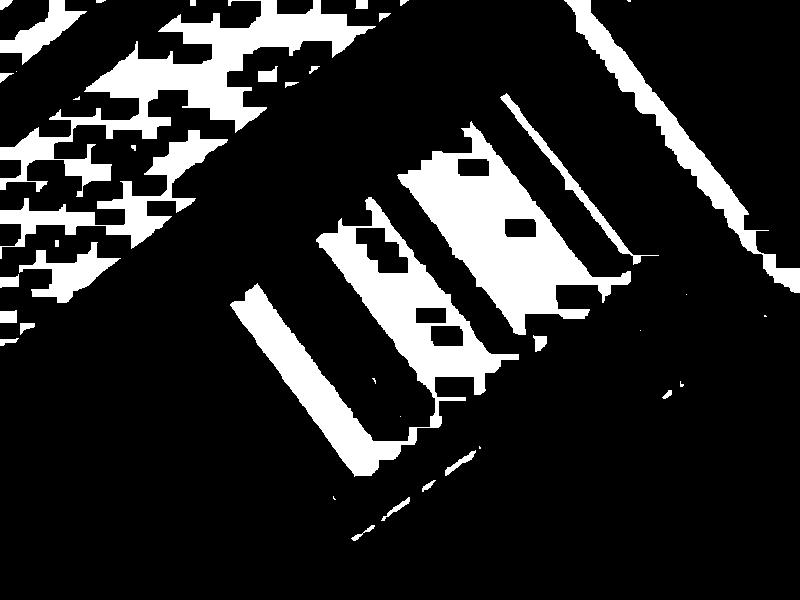
\includegraphics[width=0.4\textwidth,natwidth=800,natheight=600]{img/gradientblurfail.jpg}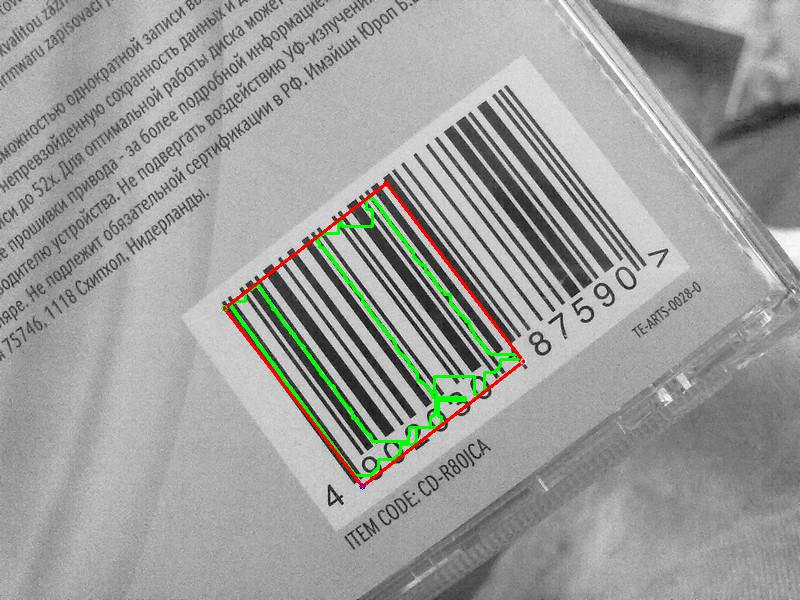
\includegraphics[width=0.4\textwidth,natwidth=800,natheight=600]{img/gradientblurfail2.jpg}
\caption{If the kernel size does not match to the barcode size Gradient+Blur fails to fully close the contour. The detected barcode is shown in red.}
\label{failgradblur}
\end{figure}

\subsubsection*{LSD}
Pros:

The LSD is still relatively fast and can reliably detect a barcode in almost every position and rotation.
\\
\\
Cons:

The LSD looks for all parallel lines. If other parallel lines are parallel to the barcode and close enough they can be added to the barcode by mistake. Disturbances like reflections can also break barcode lines and lead to exclusion valid lines.

\subsubsection*{Variation}
Pros:

Variation
\\
\\
Cons:

Variation

\subsubsection*{LSD Bound}
Pros:

The LSD Boundary Detection is extremely accurate since it test all significant lines determent by the LSD localization and returns multiple potentiality boundary points.
\\
\\
Cons:

Since it is strongly dependent on the LSD localization it fails as soon as the LSD localization fails. And since an enormous amount of lines needs to be tested the algorithms is not suited for real time applications.

\subsubsection*{Wachenfeld}
Pros:

The Wachenfeld algorithm is relatively quick since it is based on a scan line.
\\
\\
Cons:

The algorithm is strongly dependent on the quality of the preprocessing and detection of local extrema. And since the algorithm is based on a scan line it has no way to deal with broken barcodes caused by disturbances as seen in \cref{failwachenfeld}. Finally if the last segment selection steps misses the barcode can be shifted to the left or right and become unreadable.

\begin{figure}[t]
\center
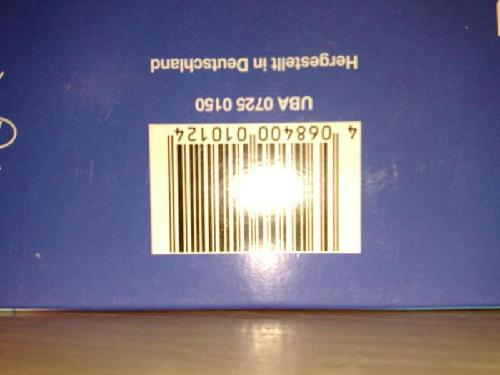
\includegraphics[width=0.4\textwidth,natwidth=800,natheight=600]{img/wachenfeldfail.jpg}
\hspace{1cm}
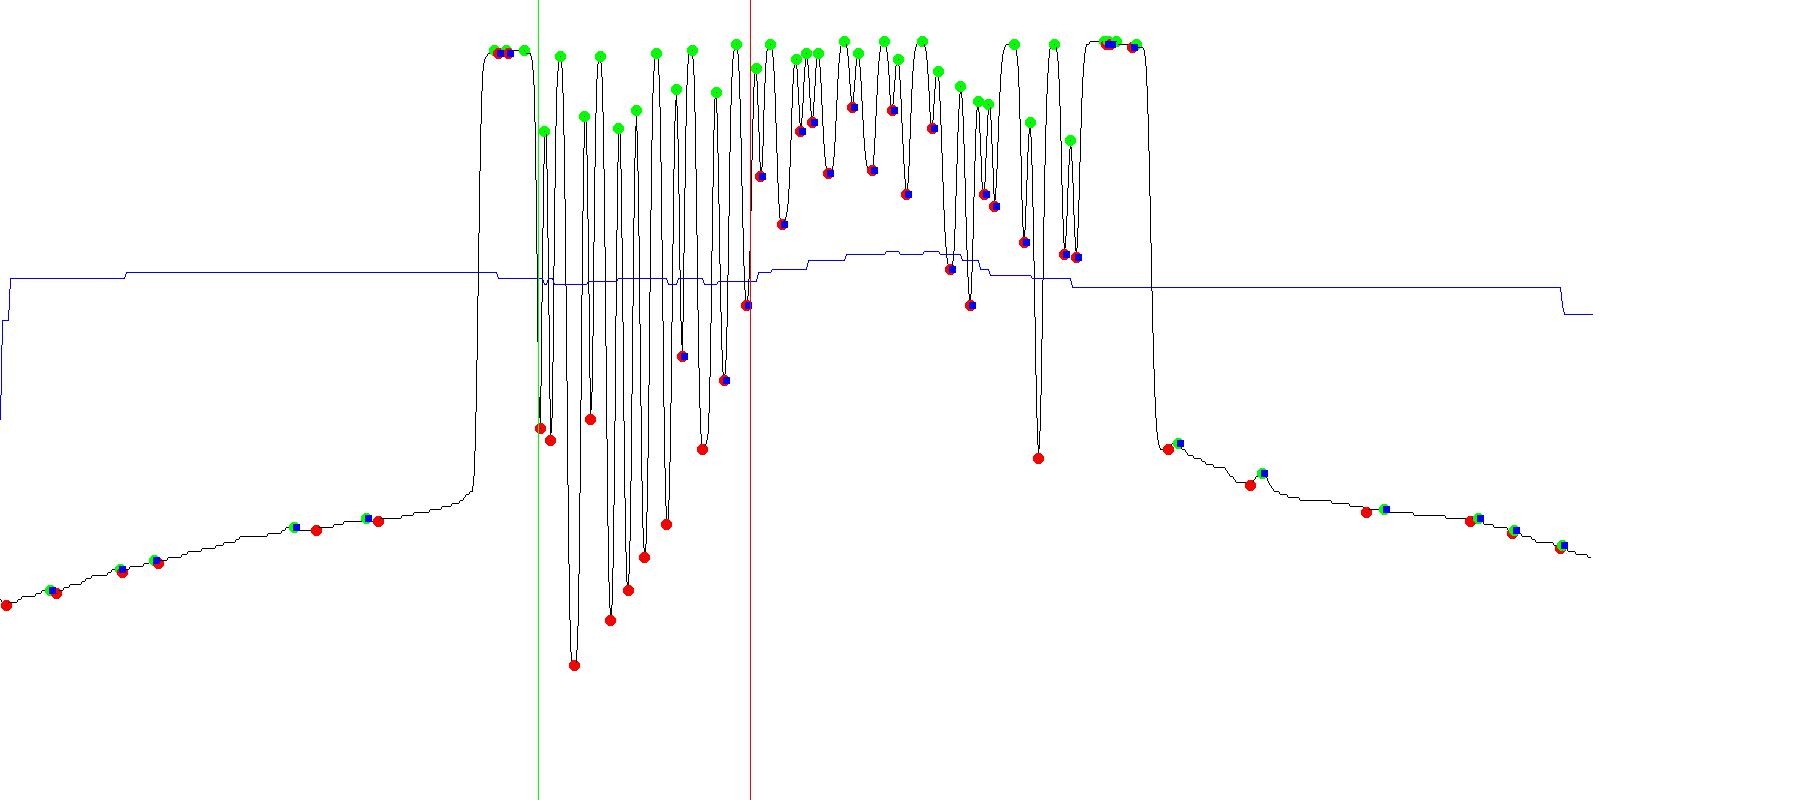
\includegraphics[width=0.4\textwidth,natwidth=1800,natheight=800]{img/wachenfeldfail2.jpg}
\caption{Preprocessin failing to apply dynamic thresholding and determining local extrema because of light reflections.}
\label{failwachenfeld}
\end{figure}
 
\subsubsection*{Template Matching}
Pros:

Since no binarization is required template matching is extremely robust against bluered barcodes. The algorithm also uses percentages to read the barcode and is therefor flexible when encountering errors. 
\\
\\
Cons:

The matching process required precomputed data to be matched against the barcode. This can take a lot of time and memory depending on the targeted accuracy. And since the template matching is based on probability it is more likely to return a false positive result than no result.

\subsection{Datasets}
The implemented algorithms were tested on three datasets.
\begin{itemize}
\item Generated Barcodes:
\begin{itemize}
\item 110 images, 300$\times$150 px, barcode only.
\item 110 images, 1000$\times$1000 px, barcodes (300$\times$150 px) randomly rotated and translated on white background.
\end{itemize}
\item WWU Muenster Barcode Database \cite{MuensterBarcodeDB} \citep{wachenfeld2008robust}:\\
1055 images, 800$\times$600 px.
\item ArteLab Dataset - Robust Angle Invariant 1D Barcode Detection \cite{ArteLabDB} \cite{zamberletti2010neural} \citep{zamberletti2013robust}:\\
2 sets of 215 images, 800$\times$600 px.
\end{itemize}

\subsection{Run-Time and Hit Rate Comparison}
The algorithms were compared over the 1055 images of the WWU Muenster Barcode Database \citep{MuensterBarcodeDB}. The programm was implemented in C++ with the help of the Qt 5.7 and OpenCV 3.1 frameworks. The test were made on a Debian 8 system with an Intel N2940 CPU, 4 Cores / 4 Threads, and 4 GB RAM. The results are shown in \cref{laufzeit}.
\\
\\
The experimental results illustrate the pros and cons of the various algorithms shown in \cref{sec:ProCon}. The Gradient+Blur algorithm performs the best in respect to speed but the worst in respect to hit rate. The simplicity of the method is directly apparent. But the listed problems cause it to miss the boundaries or even fail to detect the barcode.

Second best algorithm in speed is the Wachenfeld boundary detection. This is primary achieved through the usage of scan lines. But the unoptimized preprocessing causes the algorithm to miss the boundaries in over 40\% of tests since the dynamic thresholding fails to apply.

Both Variation Boundary Detection and LSDBounds take a very long time to detect the boundaries. This is caused by the multiple computation heavy probings of possible boundaries. But since the correct boundaries are inevitable to be probed and the algorithms produces multiple candidates both algorithms produce a high hit rate.


\begin{figure}[t]
\center
\bgroup
\def\arraystretch{1.5}
\begin{tabular}{|l|r|r|r|}
\hline
&\textbf{Errors}&\textbf{Hit rate}&\textbf{Time in sec.}\\
\hline
\textbf{Gradient + Blur}& 831& 22\%& 266\\
\hline
\textbf{LSD + Variation}& 279& 74\%& 1595\\
\hline
\textbf{LSD + LSDBounds}& 41& 97\%& 1760\\
\hline
\textbf{LSD + Wachenfeld}& 452& 56\%& 319\\
\hline
\end{tabular}
\egroup
\caption{Comparison of different algorithms on the WWU Muenster Barcode Database. All algorithms use Template Matching to read the barcode.}
\label{laufzeit}
\end{figure}
 